\documentclass[__main__.tex]{subfiles}

\begin{document}

\section{Доказательство безусловной корректности неявной разностной схемы численного решения задачи Коши для одномерного параболического уравнения}

Рассмотрим задачу Коши ($D>0$):

\begin{gather}\label{27.1}
\begin{cases}
\frac{\partial U \left(t,x\right)}{\partial t} - D \frac{\partial^2 U \left( t,x \right)}{\partial x^2} = f \left( t,x \right), \ \left(t,x\right) \in \left(0,T\right) \times \left( a;b \right) \\
U\left(0,x\right) = \mu \left(x\right), \ x \in \left[a;b\right] \\
U(t,a) = \beta_0 \left(t\right), \ U\left( t,b \right) = \beta_1 \left(t\right), \ t\in\left[0;T\right]
\end{cases}
\end{gather}

Получаем конечно-разностную схему:

\begin{figure}[h!]
	\centering
	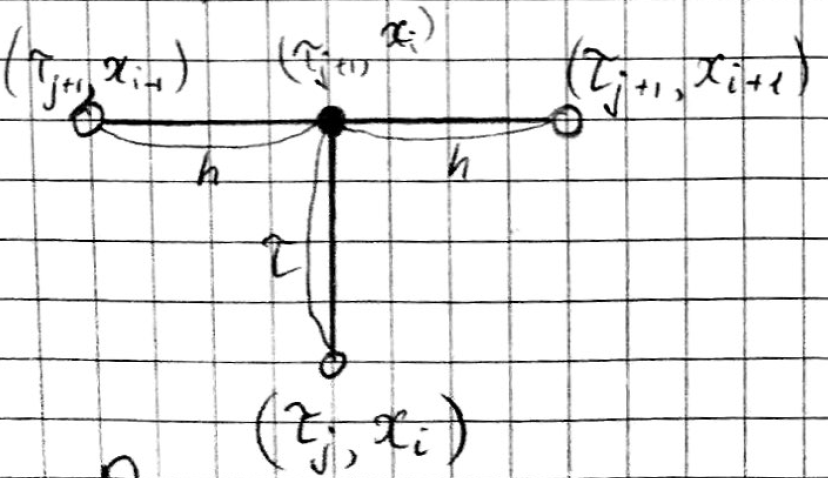
\includegraphics[width=0.03\linewidth]{img/img_27-1}
	\caption{}
	\label{img_27.1}
\end{figure}

\begin{gather}\label{27.2}
\begin{cases}
\frac{U^{j+1}_i - U^j_i}{\tau} - D \frac{U^{j+1}_{i-1} - 2 U^{j+1}_i+U^{j+1}_{i+1}}{h^2} = f^{j+1}_i, \ j = \overline{0,n-1}, \ i = \overline{1,m-1} \\
U^0_i = \mu_i, \ i = \overline{0,m}, \ \left( \mu_0 = \beta^0_1, \mu_m = \beta^0_\lambda \right) \\
U^j_0 = \beta^j_1, \ U^j_m = \beta^j_2, \ j = \overline{1,n}.
\end{cases}
\end{gather}

Для решения V задачи \ref{27.1} на сетке $C = A \times B$ получаем:

\begin{gather} \label{27.3}
\begin{cases}
\frac{V^{j+1}_i - V^j_i}{\tau} - D \frac{V^{j+1}_{i-1} - 2V^{j+1}_i +V^{j+1}_{i+1}}{h^2} = f^{j+1}_i + O \left( \tau, h^2 \right), \ j = \overline{0,n-1}, \ i = \overline{1,m-1}, \ \tau, h \rightarrow 0 \\
V^0_i = \mu_i, \ i = \overline{0,m}; \ V^j_0 = \beta^j_1, \ V^j_m = \beta^j_2, \i= \overline{0,n}.
\end{cases}
\end{gather}

Введём обозначения:

\begin{gather}\label{27.4}
\begin{cases}
V^j_i = U^j_i + \delta U^j_i, \ j=\overline{0,n}, \ i=\overline{1,m} \\
{}^>\delta U^j = [ \delta U^j_0, \delta U^j_1, ..., \delta U^j_m \rangle, \ j = \overline{0,m} \\
{}^>\delta U^0_j = {}^> O \in {}^> \mathbb{R}^{\left|B\right|} \left(B\right) \\
\delta U^j_0 = \delta U^j_m = 0, \ j = \overline{0,n} \\
{}^> \delta U = [ {}^> \delta U^0, {}^> \delta U^1, ..., {}^> \delta U^n \rangle \in {}^>\left( {}^> \mathbb{R}^{\left| B \right|} \left(B\right) \right)^{\left|A\right|} \left(A\right) \\
{}^> \varepsilon^j = \{ \varepsilon^j_0,\varepsilon^j_1, ..., \varepsilon^j_n \rangle \\
{}^\varepsilon = [ {}^>\varepsilon^0, {}^>\varepsilon^1, ..., {}^>\varepsilon^n \rangle \\
\left| \varepsilon^j_i \right| \leq \varepsilon = O \left( \tau, h^2 \right), \ h,\tau \rightarrow 0 \\
\| {}^> \varepsilon^j \|  \leq \varepsilon, \ \| {}^>\varepsilon |\ \leq \varepsilon
\end{cases}
\end{gather}

Используя обозначения \ref{27.4} и вычитая из \ref{27.3} формулы \ref{27.2} получаем:

\begin{gather}\label{27.5}
\begin{cases}
\delta U^0_i = 0, \ i = \overline{0,m} \\
\delta U^j_0 = \delta^j_m = 0, \ j = \overline{1,n} \\
\frac{\delta U^{j+1}_i - \delta U^j_i}{\tau} - D \frac{\delta U^{j+1}_{i-1} - 2\delta U^j_i + U^{j+1}_{i+1}}{h^2} = \varepsilon^{j+1}_i, \ j= \overline{0,n-1}, \ i =\overline{1,m-1}
\end{cases}
\end{gather}

Схему \ref{27.5} представим в виде:

\begin{gather}\label{27.6}
\begin{cases}
{}^> \delta U^0 = {}^> 0, \ \delta U^j_0 = \delta U^j_m = 0, \ j = \overline{1,m} \\
- \frac{D\tau}{h^2} U^{j+1}_{i-1} + \left( 1 + 2 \frac{D\tau}{h^2} \right) U^{j+1}_i - \frac{D\tau}{h^2} U^{j+1}_{i+1} = \delta U^j_i + \varepsilon^{j+1}_i, \ j = \overline{0,n-1}, \ i= \overline{1,m-1}
\end{cases}
\end{gather}

ВВедём обозначение :

\begin{gather}\label{27.7}
\begin{cases}
p = - \frac{D\tau}{h^2}, q = 1 + 2\frac{D\tau}{h^2},r = - \frac{D\tau}{h^2} \\
H = 
\left(
\begin{matrix}
1 & 0 & 0 & 0 & ... & 0 \\
p & q & r & 0 & ... & 0 \\
0 & p & q & r & ... & 0 \\
... & ... &... &... &... & \\
0 & ... & ... & p & q & r \\
0 &... & ... & 0 & 0 & 1
\end{matrix}
\right)
\end{cases}
\end{gather}

Используя обозначения \ref{27.4} и \ref{27.7}, схему \ref{27.6} представим в виде:

\begin{gather}\label{27.8}
\begin{cases}
{}^> \delta U^0 = {}^>0 \\
H \cdot {}^>\delta U^{j+1} = {}^> \delta U^j + {}^> \varepsilon^{j+1} \\
G = H^{-1}
\end{cases}
\end{gather}

где $\| H^{-1} \| = \| G \| < 1$, так как $diag\left(H\right) > 1$.

Введя обозначения:

$$
H^{-1} \cdot {}^> \varepsilon^{j+1} = G \cdot {}^>\varepsilon^{j+1} = \underline{\varepsilon}^{j+1}, \ j = \overline{0,n-1}
$$

получаем, что 

\begin{equation} \label{27.9}
\| {}^> \underline{\varepsilon}^{j+1} \| \leq \| H^{-1} \| \cdot \| {}^> \varepsilon^{j+1} \| = \| G \| \cdot \| {}^> \varepsilon^{j+1} \| < \varepsilon, \ j = \overline{0,n-1}
\end{equation}

так как $\| G \| < 1$.

Используя \ref{27.8} и \ref{27.9} получаем:

\begin{gather}\label{27.10}
\begin{cases}
{}^> \delta U^0 = {}^> 0 \\
{}^> \delta U^{j+1} = G {}^> \delta U^j + \tau \cdot {}^> \varepsilon^{j+1}, \ j = \overline{0,n-1}
\end{cases}
\end{gather}

$\| {}^> \underline{\varepsilon}^{j+1} \| < \varepsilon = 0$ и $\| G \| \leq 1$

Отсюда, как и ранее, получаем, что 

$$
\| {}^> \delta U^j \| \leq \| {}^> \delta U^0 \| + t \varepsilon \sim O \left( \tau, h^2\right) \xrightarrow[\tau, h \rightarrow 0]{} 0
$$

Следовательно, схема \ref{27.2} аппроксимирует задачу \ref{27.1} и устойчива, т.е. согласно теореме Лакса - корректна.

\paragraph{Теорема о безусловной корректности неявной схемы}
	$$
	\lim_{\tau, h \rightarrow 0} spl \left( C, {}^U \right) = V
	$$
	
	и схема \ref{27.2} корректна. $\#$

В обозначениях \ref{27.4}, \ref{27.7} и \ref{27.8} схема \ref{27.2} принимает вид: ${}^> U^0 = {}^> \mu$.

\begin{gather}\label{27.11}
\begin{cases}
H \cdot {}^> U^1 = {}^> U^0 - {}^> \beta^0 + {}^>\beta^1 + \tau {}^> f^1 \\
H \cdot {}^> U^2 = {}^> U^1 - {}^> \beta^1 + {}^>\beta^2 + \tau {}^> f^2 \\
... \\
H \cdot {}^> U^n = {}^> U^{n-1} - {}^> \beta^{n-1} + {}^>\beta^n + \tau {}^> f^n \\
\end{cases}
\end{gather}

где ${}^> \beta^0 = {}^> 0, {}^> \beta^i = [ \beta^i_1, 0 , ...,  0, \beta^i_2 \rangle$ и ${}^>f^i = [ 0, f^i_1, ..., f^i_{m-1}, 0 \rangle$ для $i = \overline{1,n}$.

Вид \ref{27.11} поясняет название "неявная схема", так как для определения ${}^>U^{i+1} \in {}^> \mathbb{R}^{\left|B\right|} \left(B\right)$ требуется решить СЛАУ с матрицей $H$ и правйо частью ${}^>U^i - {}^>\beta^i + {}^> \beta^{i+1} + \tau \cdot {}^> f^{i+1}$. Такие СЛАУ решаются методом прогонки
\end{document}
